\section{Telas}
\newpage
Nessa seção é apresentado os protótipos de como esperar o sistema da MR Telles.

Na Figura \ref{fig:2}, é demonstrado como será feita a página de acesso do sistema. Vai contar com a opção de login e cadastro como pré-requisito para acessar.

Na Figura \ref{fig:3}, é apresentada a tela de login projetada para acessar o sistema, caso o usuário já possua cadastro.

Na Figura \ref{fig:4}, está representado o formulário de cadastro projetado para criar uma conta de acesso ao sistema.

Na Figura \ref{fig:5}, é possível ver como será realizado o processo de agendamento de consultas para os usuários da plataforma após acessarem o sistema.

Na Figura \ref{fig:6}, é possível ver como é realizado o processo de administração de compromissos para os administradores/advogados da plataforma após acessarem o sistema com suas contas com permissão especial.

Na Figura \ref{fig:7}, é possível realizar o gerenciamento de consultas, onde o usuário ou administrador pode alterar a consulta mudando de dia ou excluindo-a.

Na Figura \ref{fig:8}, é apresentado o gerenciamento financeiro do sistema, onde se encontra a tabela de preços dos serviços. Todos os usuários podem acessar para ver o cálculo de quanto ficarão os seus casos.

Na Figura \ref{fig:9}, é apresentado o serviço de pagamento via Pix, onde a pessoa pode inserir o valor que necessita pagar pelos serviços da MR Telles e automaticamente um código QR Code com o valor para pagamento é gerado.

Na Figura \ref{fig:10}, é apresentado o processo de automação, onde o sistema envia mensagens automáticas para o usuário e pessoas relacionadas em determinada ação dentro do sistema. Por exemplo, quando há uma alteração de uma consulta, uma mensagem é enviada para o usuário e para o advogado responsável por essa reunião.

\begin{figure}[!ht]
    \centering
    \caption{Primeira Página}
    \label{fig:2}
    
\includegraphics[width=0.8\linewidth]{imagens/welcome.png}
\end{figure}

\begin{figure}[!ht]
    \centering
    \caption{Login}
    \label{fig:3}
     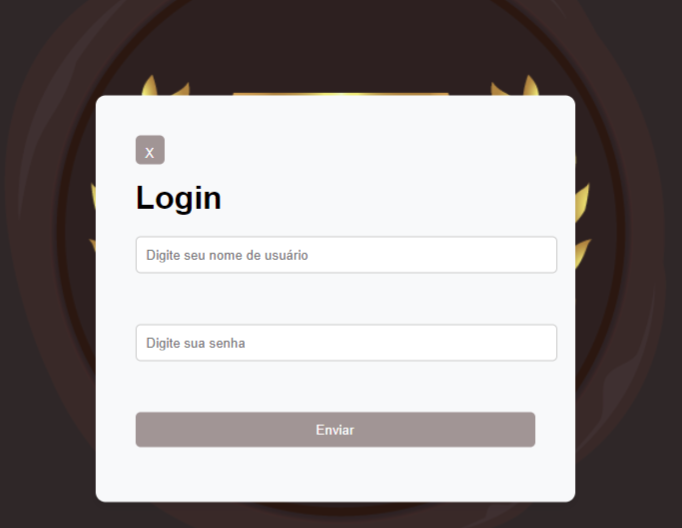
\includegraphics[width=0.8\linewidth]{imagens/login.png}
\end{figure}

\begin{figure}[!ht]
    \centering
    \caption{Cadastro}
    \label{fig:4}
    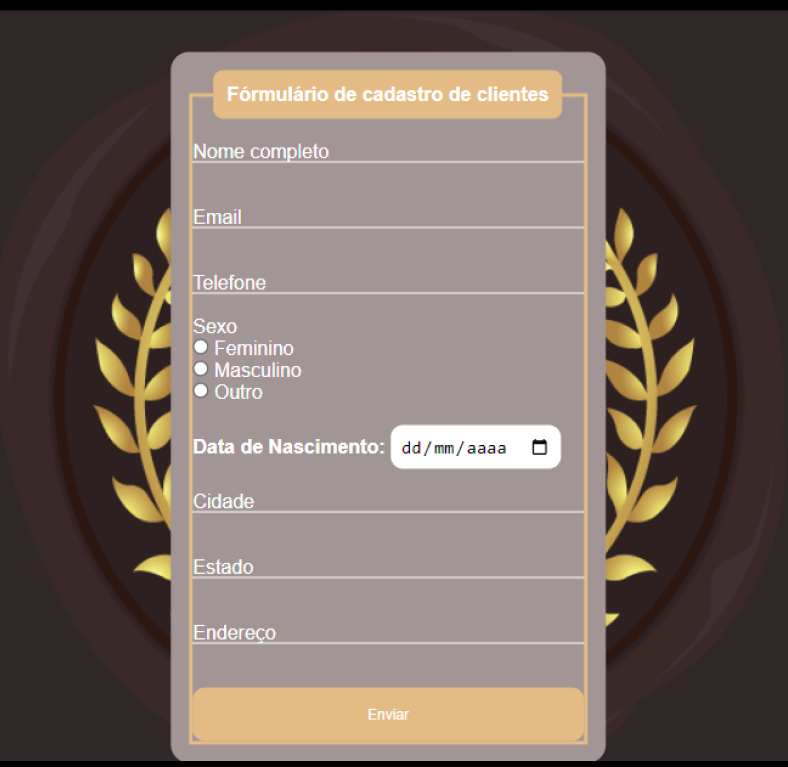
\includegraphics[width=0.8\linewidth]{imagens/cadastro.png}
\end{figure}

\begin{figure}[!ht]
    \centering
    \caption{Agendamentos}
    \label{fig:5}
    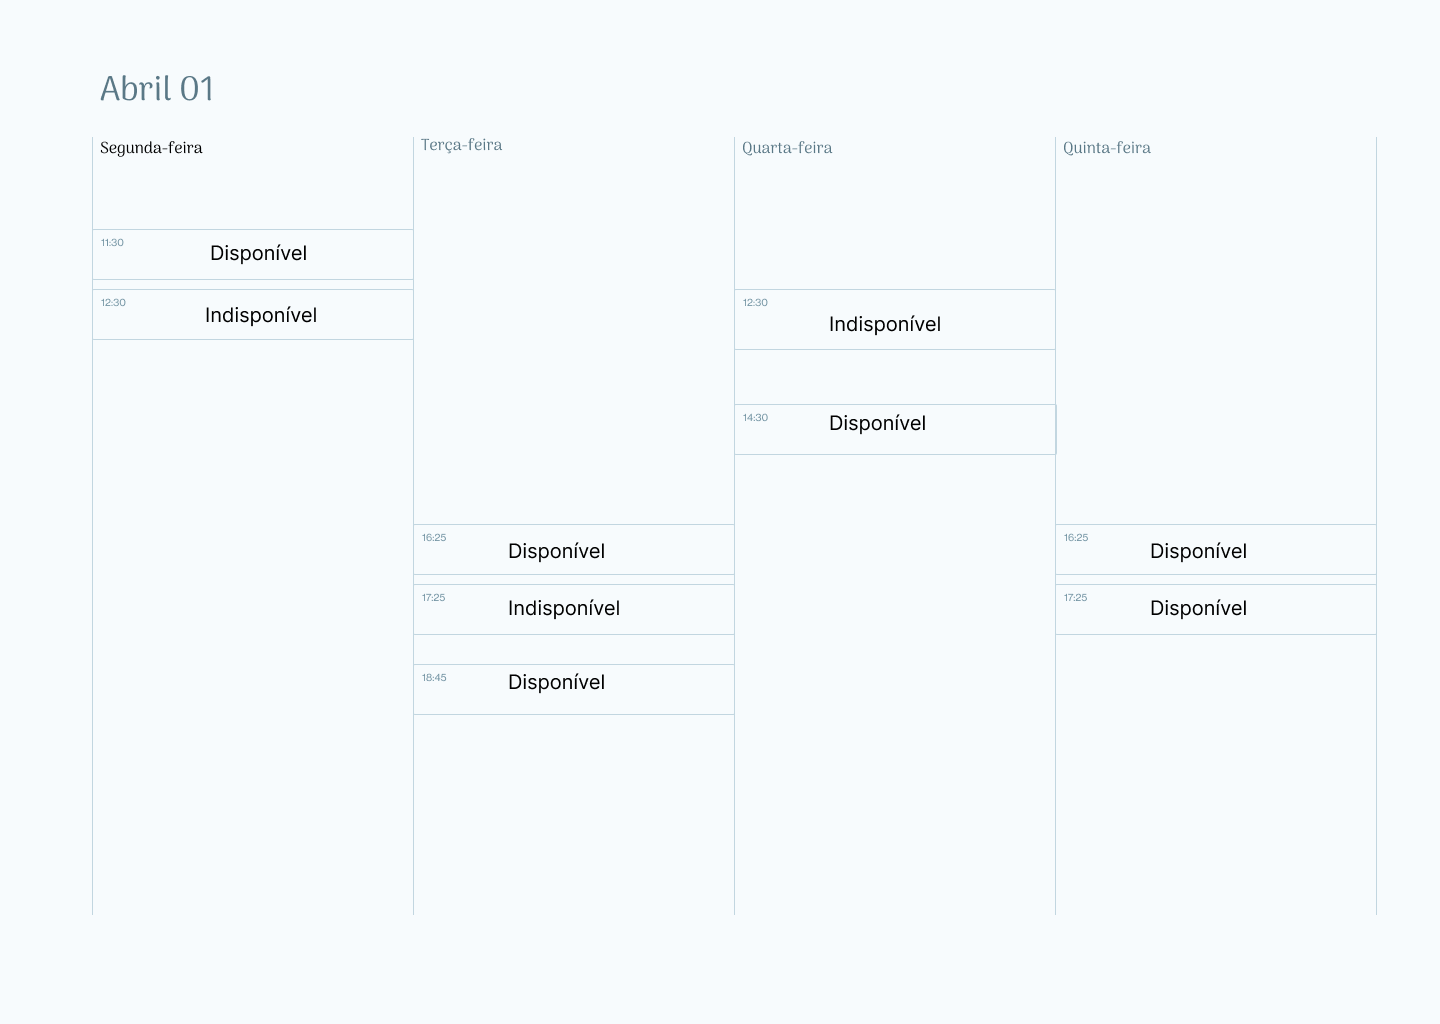
\includegraphics[width=0.8\linewidth]{imagens/Gerenciar agendamento.png}
\end{figure}

\begin{figure}[!ht]
    \centering
    \caption{Administrar Compromissos}
    \label{fig:6}
    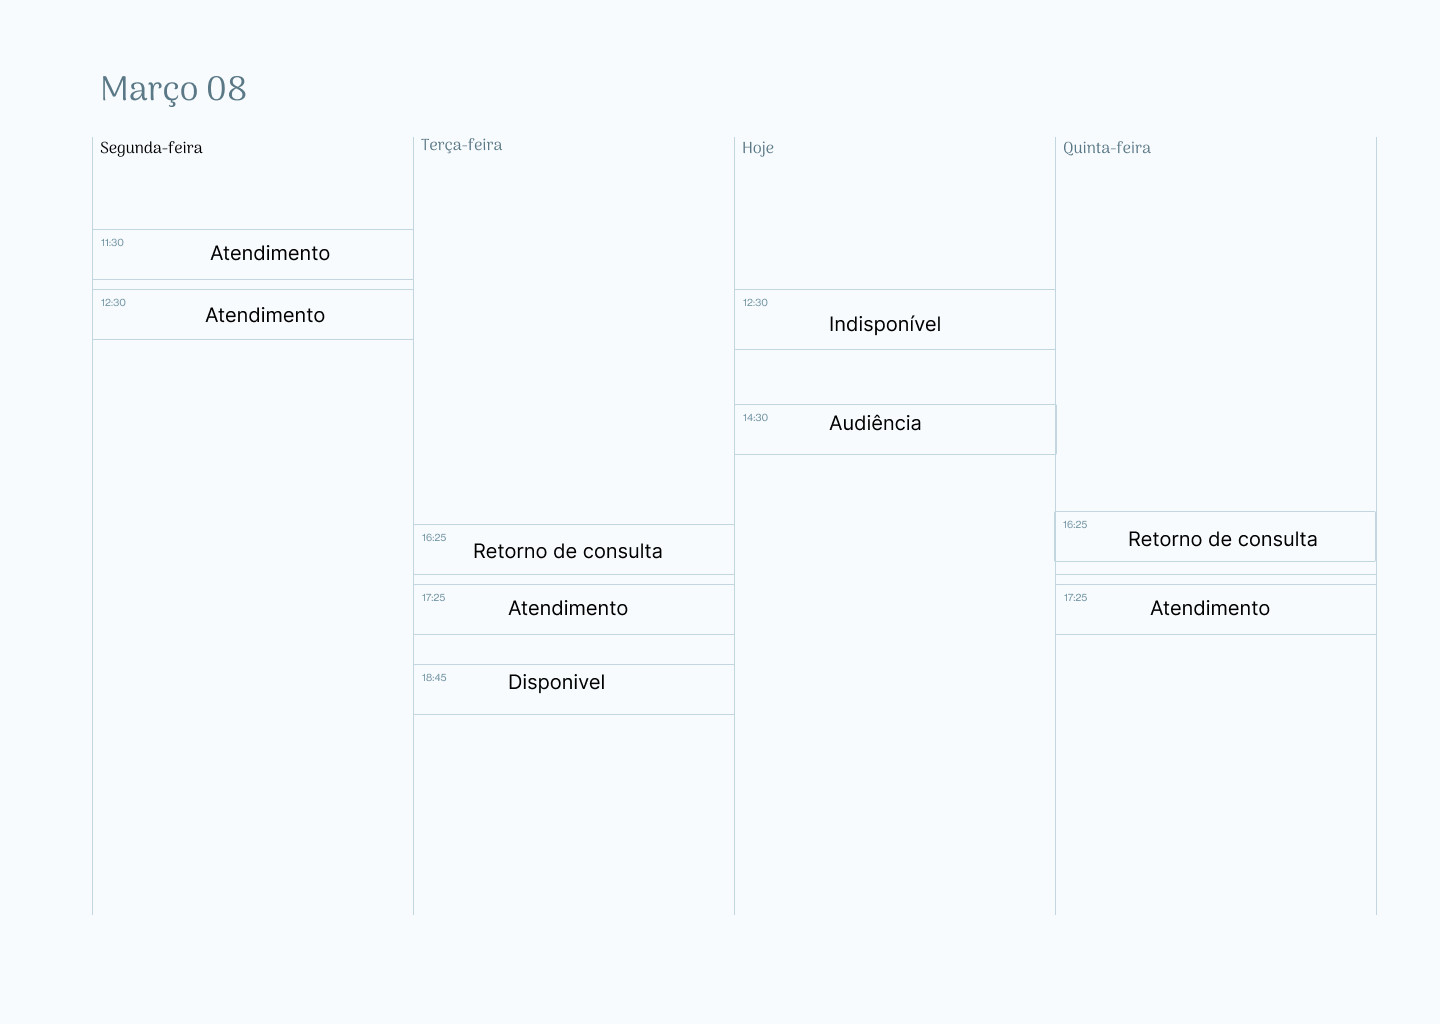
\includegraphics[width=0.8\linewidth]{imagens/Administrar compromissos.png}
\end{figure}

\begin{figure}[!ht]
    \centering
    \caption{Gerenciar Consultas}
    \label{fig:7}
    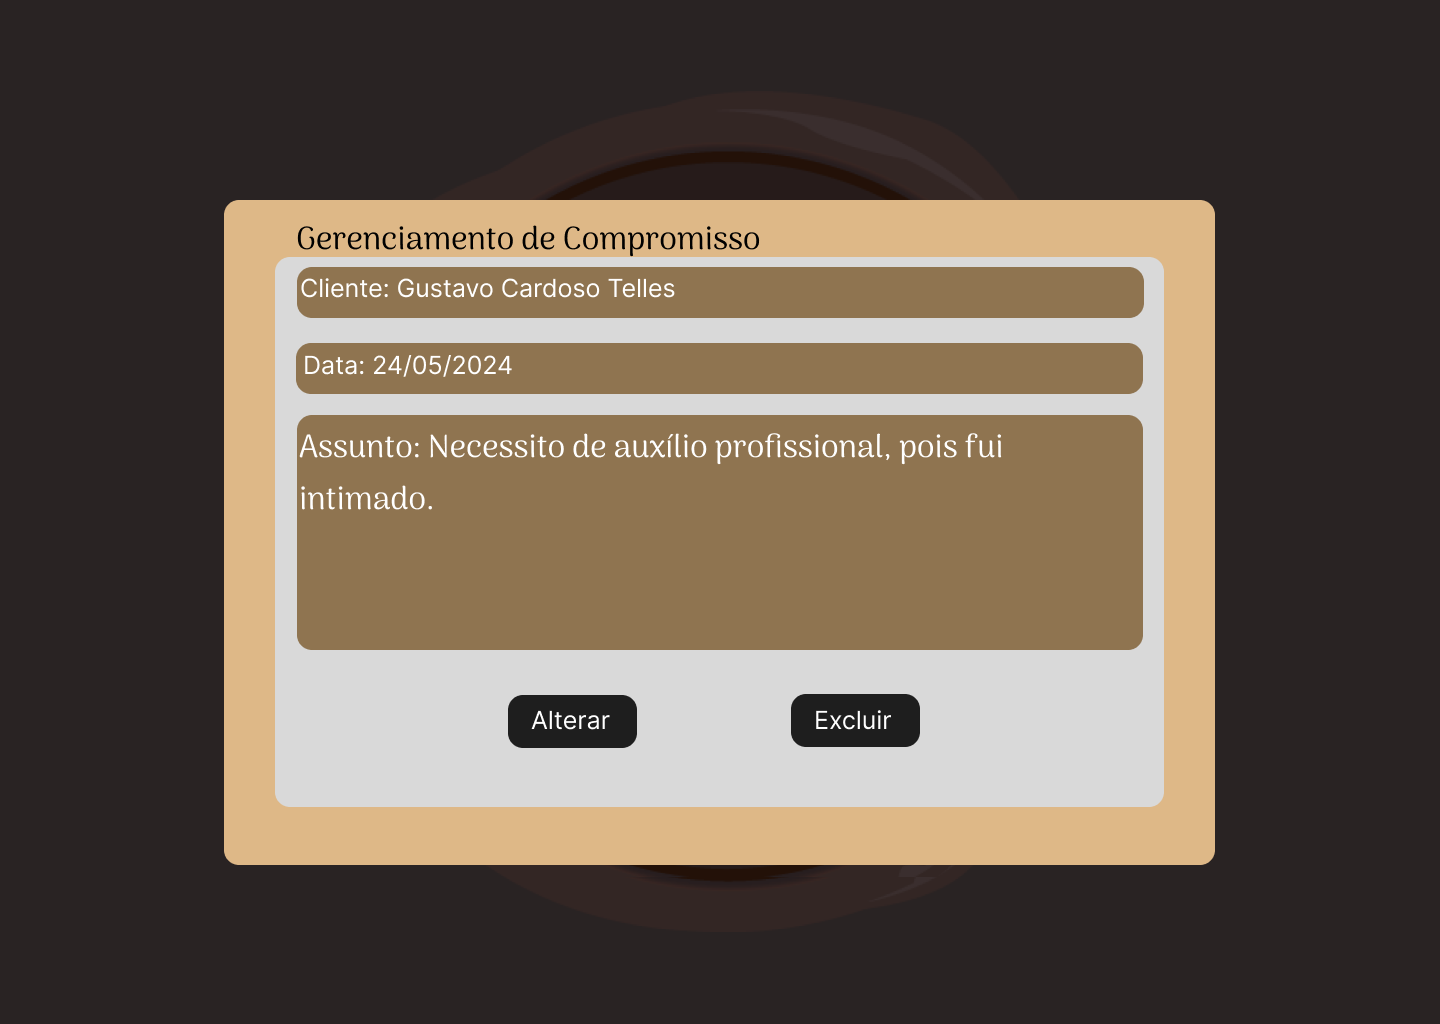
\includegraphics[width=0.8\linewidth]{imagens/Administrar consulta.png}
\end{figure}

\begin{figure}[!ht]
    \centering
    \caption{Financeiro}
    \label{fig:8}
    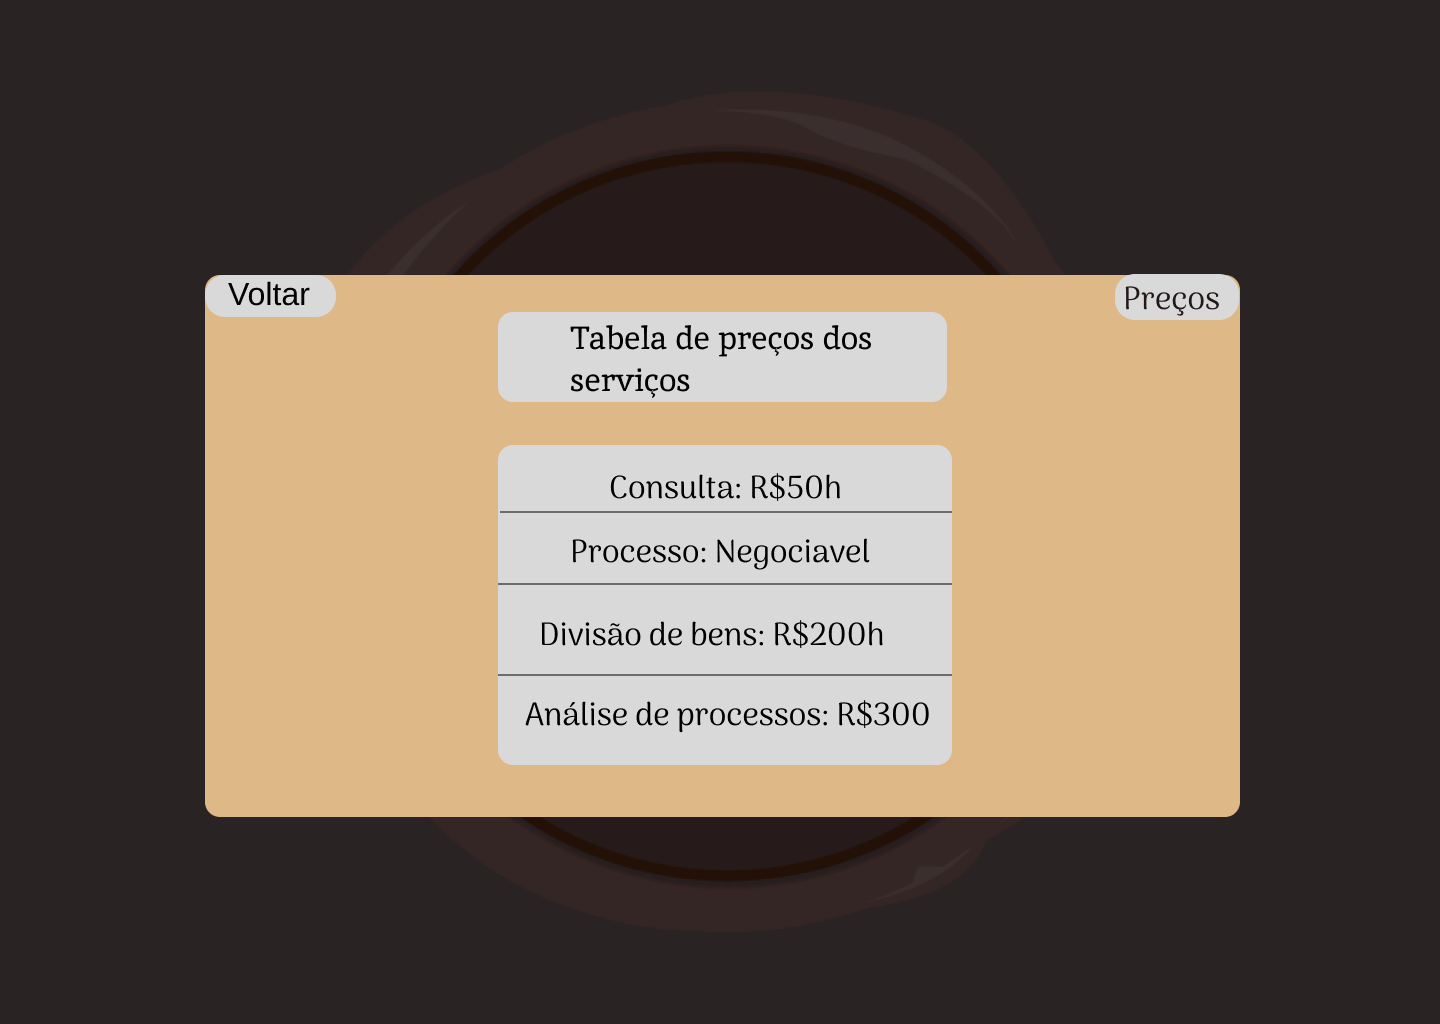
\includegraphics[width=0.8\linewidth]{imagens/Financeiro.png}
\end{figure}

\begin{figure}[!ht]
    \centering
    \caption{Pagamento}
    \label{fig:9}
    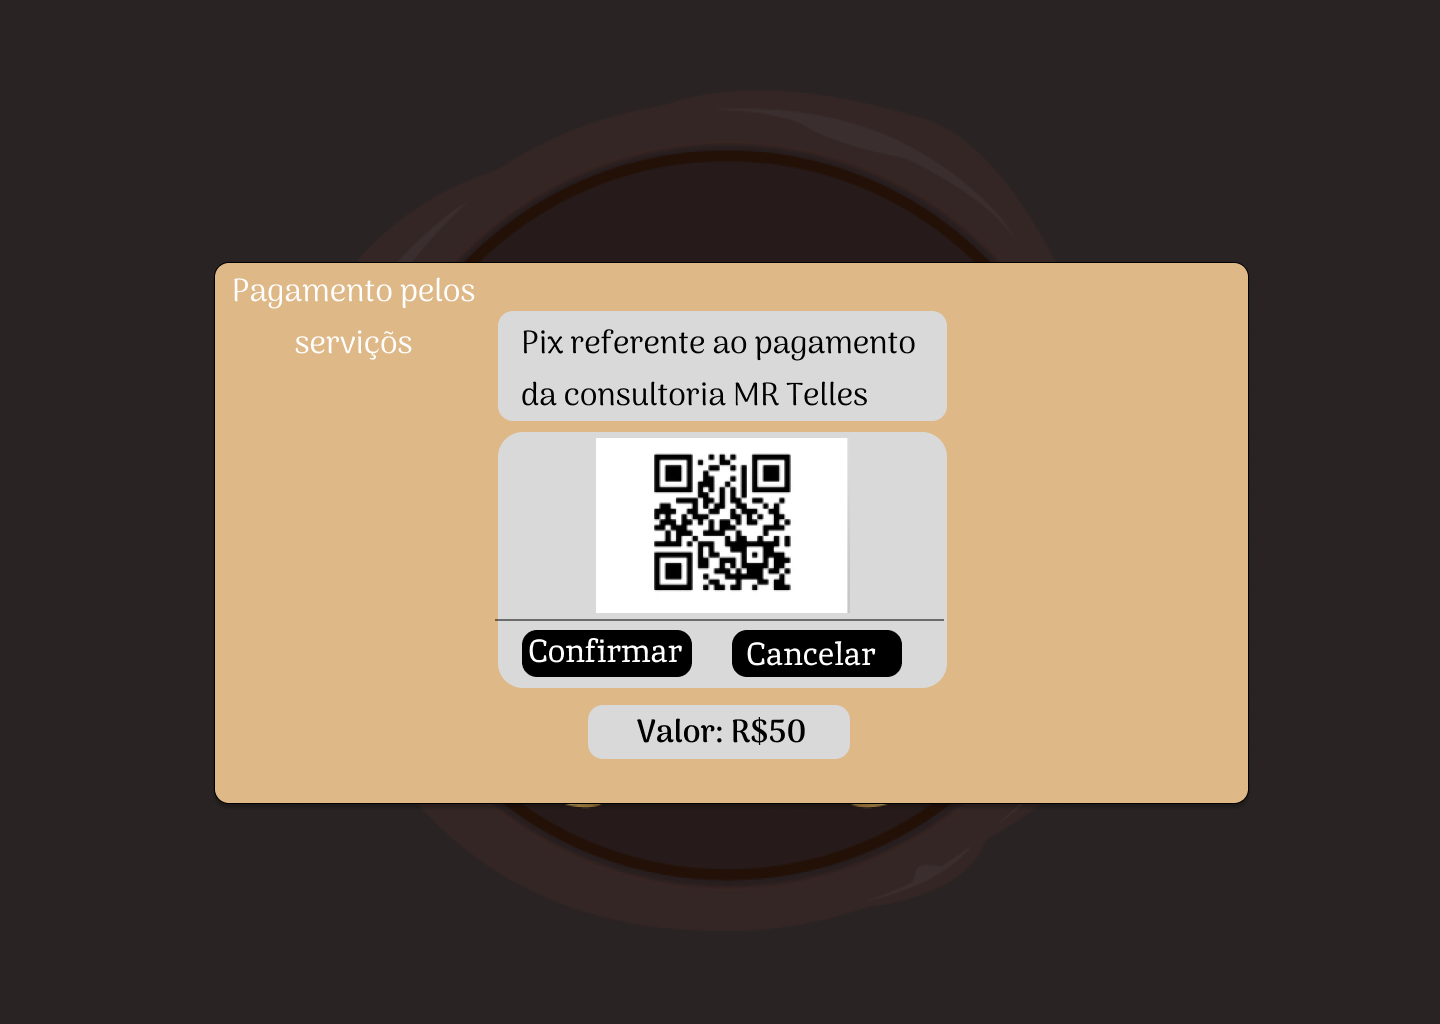
\includegraphics[width=0.8\linewidth]{imagens/Pagamento.png}
\end{figure}

\begin{figure}[!ht]
    \centering
    \caption{Automação}
    \label{fig:10}
    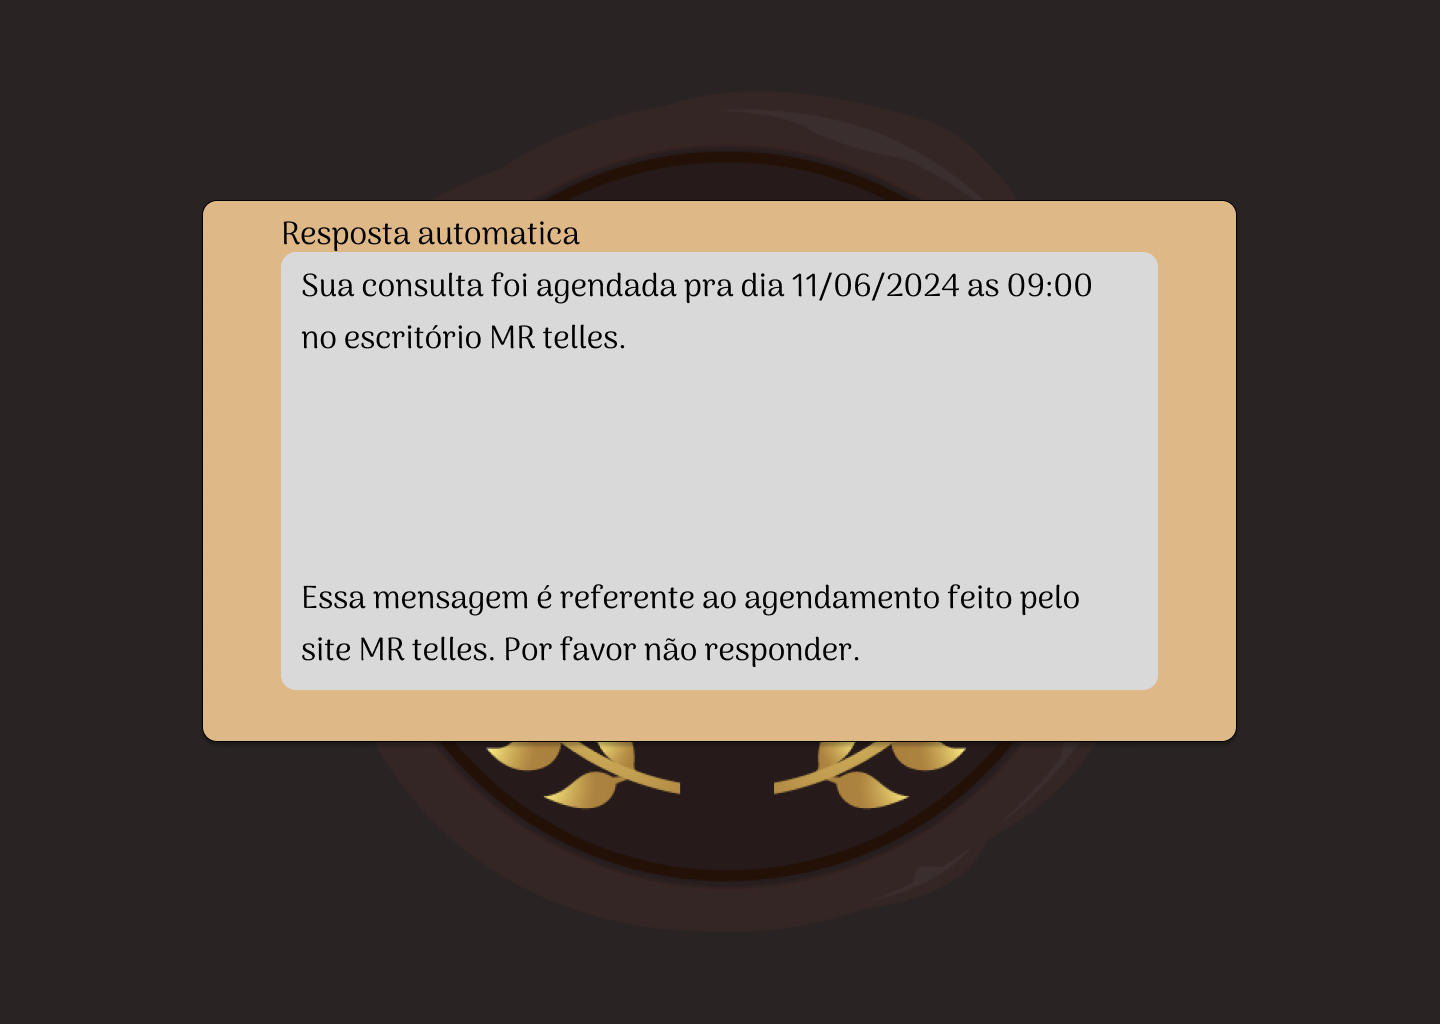
\includegraphics[width=0.8\linewidth]{imagens/Automação.png}
\end{figure}